\documentclass[11pt, aspectratio=169]{beamer}

% LuaLaTeXで日本語を使うための必須パッケージ (English slides can still be compiled with luatexja if kept, or removed if pure English engine is used)
\usepackage{luatexja}

% 便利な追加パッケージ
\usepackage{booktabs}   % 表の罫線
\usepackage{tikz}       % 図形描画
\usepackage{listings}   % ソースコード挿入
\lstset{
  basicstyle=\ttfamily\scriptsize,
  frame=single,
  breaklines=true,
  numbers=left,
  numberstyle=\tiny
}

% テーマとカラーテーマの設定
\usetheme{Madrid}
\usecolortheme{orchid}

% セクション開始時の自動表紙（扉絵）設定
\AtBeginSection[]{
  \begin{frame}
    \vfill
    \centering
    \begin{beamercolorbox}[sep=8pt,center,shadow=true,rounded=true]{title}
      \usebeamerfont{title}\insertsectionhead\par%
    \end{beamercolorbox}
    \vfill
  \end{frame}
}

% サブセクション開始時の自動表紙（扉絵）設定
\AtBeginSubsection[]{
  \begin{frame}{\insertsectionhead}
    \tableofcontents[currentsection, currentsubsection, subsectionstyle=show/shaded/hide]
  \end{frame}
}

% タイトル情報
\title{Report on Jamming Simulation Environment and Execution of Basic Jamming in Pyjama}
\subtitle{Jamming Signals}
\author{Student ID: 1280391 \\ Name: Natsuka Hosokawa}
\institute{Kochi University of Technology}
\date{\today}

\begin{document}

% タイトルスライド
\begin{frame}
  \titlepage
\end{frame}

% 目次スライド
\begin{frame}{Table of Contents}
  \tableofcontents
\end{frame}

% ==========================================
% ここから本文
% ==========================================

\section{Report on Server Environment Setup}

\begin{frame}{Server Environment}
  \begin{itemize}
    \item \textbf{Base OS}: \texttt{Ubuntu 22.04 LTS} (Stable Release)
    \item \textbf{Development Language}: \texttt{Python 3.10} (OS Standard Package)
    \item \textbf{GPU Environment (\texttt{TensorFlow 2.10} Compliant)}
    \begin{itemize}
      \item \texttt{CUDA Toolkit 11.2}
      \item \texttt{cuDNN 8.1.1}
    \end{itemize}
    \item \textbf{Objective}: To safely and reliably reproduce the legacy \texttt{GPU} computing environment required by the \texttt{Pyjama} simulator within a modern container.
  \end{itemize}
  \begin{alertblock}{Important Note}
    This environment was forcefully adapted to the current server's \texttt{GPU} infrastructure. If migrating to a different environment in the future, there is a high probability that significant changes will be required.
    \end{alertblock}
\end{frame}

\section{Execution of Basic Jamming}

\subsection{Overview of Basic Jamming}

\begin{frame}{Execution Overview of Basic Jamming}
  \begin{itemize}
    \item \textbf{Jamming Type}: Basic Jamming ($-3\text{ dB}$ jamming signal)
    \item \textbf{Execution Method}: Generation of jamming signals in an urban scenario on the \texttt{Pyjama} simulator.
    \item \textbf{Objective}: To quantitatively evaluate the impact of jamming signals on the Bit Error Rate (\texttt{BER}) of the communication.
  \end{itemize}
\end{frame}

\subsection{Results of Basic Jamming}

\begin{frame}{Measurement Results under Basic Jamming ($-3\text{ dB}$) Environment}
  \begin{table}[htbp]
    \centering
    \scriptsize 
    \begin{tabular}{rrr}
      \toprule
      EbNo [dB] & BER & BLER \\
      \midrule
      $-5.000$ & $1.3472 \times 10^{-1}$ & $1.0000$ \\
      $-3.667$ & $1.1727 \times 10^{-1}$ & $1.0000$ \\
      $-2.333$ & $8.3861 \times 10^{-2}$ & $1.0000$ \\
      $-1.000$ & $5.7059 \times 10^{-2}$ & $1.0000$ \\
      $0.333$ & $4.4591 \times 10^{-2}$ & $1.0000$ \\
      $1.667$ & $4.1223 \times 10^{-2}$ & $1.0000$ \\
      $3.000$ & $2.3917 \times 10^{-2}$ & $9.9375 \times 10^{-1}$ \\
      $4.333$ & $2.3111 \times 10^{-2}$ & $9.1875 \times 10^{-1}$ \\
      $5.667$ & $1.4810 \times 10^{-2}$ & $7.6250 \times 10^{-1}$ \\
      $7.000$ & $1.6760 \times 10^{-2}$ & $7.4375 \times 10^{-1}$ \\
      $8.333$ & $1.2167 \times 10^{-2}$ & $6.2500 \times 10^{-1}$ \\
      $9.667$ & $1.0692 \times 10^{-2}$ & $4.6250 \times 10^{-1}$ \\
      $11.000$ & $8.8928 \times 10^{-3}$ & $3.4375 \times 10^{-1}$ \\
      $12.333$ & $5.7210 \times 10^{-3}$ & $2.8125 \times 10^{-1}$ \\
      $13.667$ & $3.1993 \times 10^{-3}$ & $2.3125 \times 10^{-1}$ \\
      $15.000$ & $2.6723 \times 10^{-3}$ & $1.2500 \times 10^{-1}$ \\
      \bottomrule
    \end{tabular}
  \end{table}
\end{frame}

\begin{frame}{BER Trend under Basic Jamming ($-3\text{ dB}$) Environment}
  \begin{figure}[htbp]
    \centering
    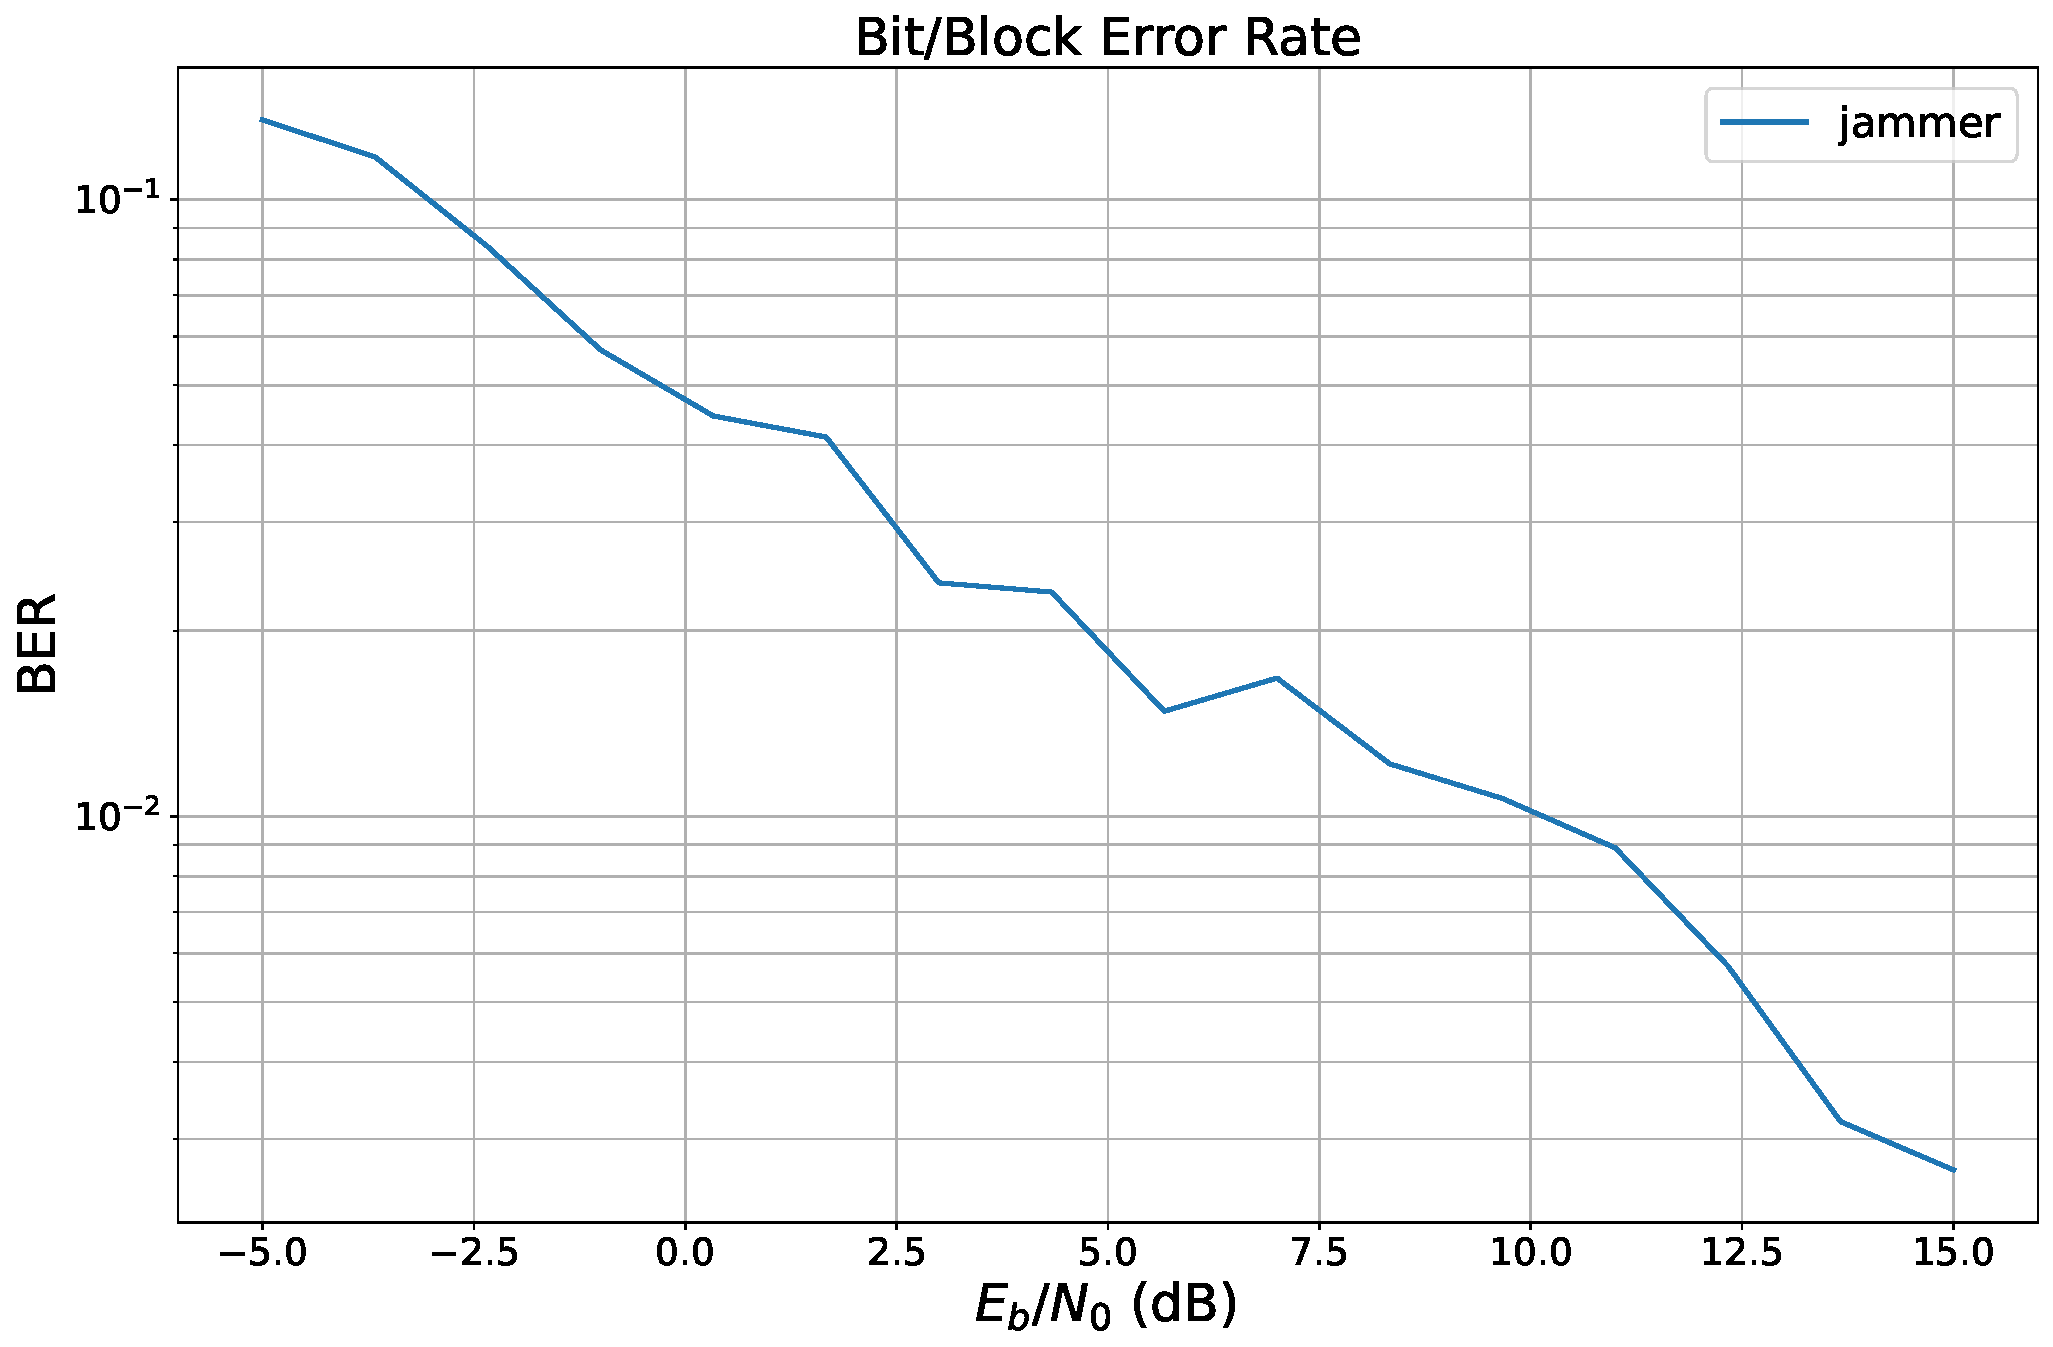
\includegraphics[width=0.7\linewidth]{img1.pdf}
    \caption{Simulation results of BER and BLER vs. EbNo (without MASH applied)}
    \label{fig:ber_result}
  \end{figure}
\end{frame}

\section{Conclusion and Future Work}

\begin{frame}{Conclusion and Future Work}
  \begin{itemize}
    \item \textbf{Achievement of Environment Setup}
    \begin{itemize}
      \item Successfully and completely reproduced the legacy \texttt{GPU} environment (e.g., \texttt{TensorFlow 2.10}) required to run the \texttt{Pyjama} simulator on a container.
    \end{itemize}
    \item \textbf{Confirmation of Basic Jamming ($-3\text{ dB}$) Impact}
    \begin{itemize}
      \item Conducted baseline measurements using the \texttt{POS} mitigation system.
      \item Confirmed the theoretical behavior where the communication error rates (\texttt{BER/BLER}) decrease as the signal strength (\texttt{EbNo}) increases, due to the relative decline in the jammer's influence (\texttt{JSR}).
    \end{itemize}
    \item \textbf{Future Work}
    \begin{itemize}
      \item Implement "\texttt{MASH}", a more advanced multi-antenna mitigation algorithm, within this environment.
      \item Compare the simulation results between \texttt{POS} and \texttt{MASH} applications to evaluate the differences in mitigation performance.
    \end{itemize}
  \end{itemize}
\end{frame}

\end{document}